
\section*{Разложение на смещение и разброс}


\subsection*{Теория}

Допустим, у нас есть некоторая выборка, на которой линейные методы работают лучше решающих деревьев с точки зрения ошибки на контроле. Почему это так? Чем можно объяснить превосходство определённого метода обучения? Оказывается, ошибка любой модели складывается из трёх факторов: сложности самой выборки, схожести модели с истинной зависимостью ответов от объектов в выборке, и богатства семейства, из которого выбирается конкретная модель. Между этими факторами существует некоторый баланс, и уменьшение одного из них приводит к увеличению другого. Такое разложение ошибки носит название разложения на смещение и разброс, и его формальным выводом мы сейчас займёмся.

\vspace*{0.4cm}

Пусть задана выборка $X = (x_i, y_i)_{i=1}^n$ с вещественными ответами $y_i \in \mathbb{R}$ (рассматриваем задачу регрессии). Будем считать, что на пространстве всех объектов и ответов $X \times Y$ существует распределение $p(x, y)$, из которого сгенерирована выборка $X$ и ответы на ней.

Рассмотрим квадратичную функцию потерь
\[
L(y, a) = (y - a(x))^2
\]
и соответствующий ей среднеквадратичный риск
\[
R(a) = \mathbb{E}_{x, y} \left[ (y - a(x))^2 \right] = \int_{X} \int_{Y} p(x, y) (y - a(x))^2 dxdy.
\]

Данный функционал усредняет ошибку модели в каждой точке пространства $x$ и для каждого возможного ответа $y$, причём вклад пары $(x, y)$, по сути, пропорционален вероятности получить её в выборке $p(x, y)$. Разумеется, на практике мы не можем вычислить данный функционал, поскольку распределение $p(x, y)$ неизвестно. Тем не менее, в теории он позволяет измерить качество модели на всех возможных объектах, а не только на наблюдённой выборке.

\subsection*{Задание}

Покажите, что минимум среднеквадратичного риска достигается на функции, возвращающей условное математическое ожидание ответа при фиксированном объекте.

\[
a_*(x) = \mathbb{E}[y \mid x] = \int_Y y p(y \mid x) dy = \arg \min_a R(a).
\]

Иными словами покажите, что мы должны провести «взвешенное голосование» по всем возможным ответам, при этом веса ответа равны апостериорной вероятности.

\subsection*{Решение}

Преобразуем функцию потерь:

\[
L(y, a(x)) = (y - a(x))^2 = (y - \mathbb{E}(y \mid x) + \mathbb{E}(y \mid x) - a(x))^2 =
\]
\[
= (y - \mathbb{E}(y \mid x))^2 + 2(y - \mathbb{E}(y \mid x))(\mathbb{E}(y \mid x) - a(x)) + (\mathbb{E}(y \mid x) - a(x))^2.
\]

Подставляя её в функционал среднеквадратичного риска, получаем:

\[
R(a) = \mathbb{E}_{x,y}[L(y, a(x))] =
\]
\[
= \mathbb{E}_{x,y}[(y - \mathbb{E}(y \mid x))^2] + \mathbb{E}_{x,y}[(\mathbb{E}(y \mid x) - a(x))^2] +
2 \mathbb{E}_{x,y}[(y - \mathbb{E}(y \mid x))(\mathbb{E}(y \mid x) - a(x))].
\]

Разберёмся сначала с последним слагаемым. Перейдём от матожидания \(\mathbb{E}_{x,y}[f(x, y)]\) к цепочке матожиданий:

\[
\mathbb{E}_x \mathbb{E}_y[f(x, y) \mid x] = \int_X \left( \int_Y f(x, y) p(y \mid x) dy \right) p(x) dx
\]

и заметим, что величина \((\mathbb{E}(y \mid x) - a(x))\) не зависит от \(y\), и поэтому её можно вынести за матожидание по \(y\):

\[
\mathbb{E}_x \mathbb{E}_y \left[ (y - \mathbb{E}(y \mid x))(\mathbb{E}(y \mid x) - a(x)) \mid x \right] =
\]
\[
= \mathbb{E}_x \left( (\mathbb{E}(y \mid x) - a(x)) \mathbb{E}_y \left[ (y - \mathbb{E}(y \mid x)) \mid x \right] \right) =
\]
\[
= \mathbb{E}_x \left( (\mathbb{E}(y \mid x) - a(x)) (\mathbb{E}_y[y \mid x] - \mathbb{E}_y \mathbb{E}(y \mid x)) \right) =
\]
\[
= 0.
\]

Получаем, что функционал среднеквадратичного риска имеет вид:

\[
R(a) = \mathbb{E}_{x,y}(y - \mathbb{E}(y \mid x))^2 + \mathbb{E}_{x,y}((\mathbb{E}(y \mid x) - a(x))^2).
\]

От алгоритма \(a(x)\) зависит только второе слагаемое, и оно достигает своего минимума, если \(a(x) = \mathbb{E}(y \mid x)\). Таким образом, оптимальная модель регрессии для квадратичной функции потерь имеет вид:

\[
a_*(x) = \mathbb{E}(y \mid x) = \int_Y y p(y \mid x) dy.
\]

Что и требовалось показать.


\subsection*{Теория}

Для того, чтобы построить идеальную функцию регрессии, необходимо знать распределение на объектах и ответах $p(x, y)$, что, как правило, невозможно. На практике вместо этого выбирается некоторый \emph{метод обучения} $\mu : (\mathbb{X} \times \mathbb{Y})^\ell \to A$, который произвольной обучающей выборке ставит в соответствие некоторый алгоритм из семейства $A$. В качестве меры качества метода обучения можно взять усредненный по всем выборкам среднеквадратичный риск алгоритма, выбранного методом $\mu$ по выборке:
\newpage
\[
    L(\mu) = \mathbb{E}_X \left[ \mathbb{E}_{x, y} \left[ \left( y - \mu(X)(x) \right)^2 \right] \right] = \tag{1}
\]
\[
    =\int_{(\mathbb{X} \times \mathbb{Y})^\ell} \int_{\mathbb{X} \times \mathbb{Y}} (y - \mu(X)(x))^2
    p(x, y) \prod_{i=1}^\ell p(x_i, y_i) dx dy dx_1 dy_1 \ldots dx_\ell dy_\ell.
\]

Здесь матожидание $\mathbb{E}_X[\cdot]$ берется по всем возможным выборкам $\{(x_1, y_1), \ldots, (x_\ell, y_\ell)\}$ из распределения $\prod_{i=1}^\ell p(x_i, y_i)$.

Обратим внимание, что результатом применения метода обучения $\mu(X)$ к выборке $X$ является модель, поэтому правильно писать $\mu(X)(x)$. Но это довольно громоздкая запись, поэтому будем везде дальше писать просто $\mu(X)$, но не будем забывать, что это функция, зависящая от объекта $x$.

Среднеквадратичный риск на фиксированной выборке $X$ можно расписать как:
\[
\mathbb{E}_{x, y} \left[ \left( y - \mu(X) \right)^2 \right] =
\mathbb{E}_{x, y} \left[ \left( y - \mathbb{E}[y \mid x] \right)^2 \right] +
\mathbb{E}_{x, y} \left[ \left( \mathbb{E}[y \mid x] - \mu(X) \right)^2 \right].
\]

\subsection*{Задание}

Подставим это представление в (1):
\[
L(\mu) = \mathbb{E}_X \left[ \mathbb{E}_{x,y} \left[ \left( y - \mathbb{E}[y \mid x] \right)^2 \right]
+ \mathbb{E}_{x,y} \left[ \left( \mathbb{E}[y \mid x] - \mu(X) \right)^2 \right] \right] =
\]
\[
= \mathbb{E}_{x,y} \left[ \left( y - \mathbb{E}[y \mid x] \right)^2 \right]
+ \mathbb{E}_{x,y} \left[ \mathbb{E}_X \left[ \left( \mathbb{E}[y \mid x] - \mu(X) \right)^2 \right] \right]. \tag{2}
\]

Преобразуем второе слагаемое:
\[
\mathbb{E}_{x,y} \left[
\mathbb{E}_X \left[ \left( \mathbb{E}[y \mid x] - \mu(X) \right)^2 \right] \right] = \]
\[
= \mathbb{E}_{x,y} \left[
\mathbb{E}_X \left[ \left( \mathbb{E}[y \mid x] -
\mathbb{E}_X[\mu(X)] + \mathbb{E}_X[\mu(X)] - \mu(X) \right)^2 \right] \right] =
\]
\[
= \mathbb{E}_{x,y} \left[
\mathbb{E}_X \left[ \left( \mathbb{E}[y \mid x] - \mathbb{E}_X[\mu(X)] \right)^2 \right] \right]
+ \mathbb{E}_{x,y} \left[
\mathbb{E}_X \left[ \left( \mathbb{E}_X[\mu(X)] - \mu(X) \right)^2 \right] \right] +
\tag{3}\]
\[
+ 2 \mathbb{E}_{x,y} \left[
\mathbb{E}_X \left[ \left( \mathbb{E}[y \mid x] - \mathbb{E}_X[\mu(X)] \right)
\left( \mathbb{E}_X[\mu(X)] - \mu(X) \right) \right] \right].
\]

Покажите, что последнее слагаемое обращается в нуль.

\subsection*{Решение}

Покажем, что последнее слагаемое обращается в нуль:
\[
\mathbb{E}_X \left[ \left( \mathbb{E}[y \mid x] - \mathbb{E}_X \left[ \mu(X) \right] \right)
\left( \mathbb{E}_X \left[ \mu(X) \right] - \mu(X) \right) \right] =
\]
\[
= \left( \mathbb{E}[y \mid x] - \mathbb{E}_X \left[ \mu(X) \right] \right)
\mathbb{E}_X \left[ \mathbb{E}_X \left[ \mu(X) \right] - \mu(X) \right] =
\]
\[
= \left( \mathbb{E}[y \mid x] - \mathbb{E}_X \left[ \mu(X) \right] \right)
\left[ \mathbb{E}_X \mu(X) - \mathbb{E}_X \mu(X) \right] =
\]
\[
= 0.
\]

\subsection*{Задание}

Используя результаты предыдущих задач и подставляя (3) в (2) получите выражение для $L(\mu)$, укажите слагаемые, отвечающие за \emph{смещение}, \emph{шум} и \emph{разброс}.

\newpage

\subsection*{Решение}

Подставим выражение (3) в (2), учитывая результаты предыдущих задач:

\[
L(\mu) = \underbrace{\mathbb{E}_{x, y} \left[ \left( y - \mathbb{E}[y \mid x] \right)^2 \right]}_{\text{шум}}
+ \underbrace{\mathbb{E}_x \left[ \left( \mathbb{E}_X [\mu(X)] - \mathbb{E}[y \mid x] \right)^2 \right]}_{\text{смещение}}
+ \underbrace{\mathbb{E}_x \left[ \mathbb{E}_X \left[ \left( \mu(X) - \mathbb{E}_X[\mu(X)] \right)^2 \right] \right]}_{\text{разброс}}.
\]

Рассмотрим подробнее компоненты полученного разложения ошибки. Первая компонента характеризует \emph{шум} (\emph{noise}) в данных и равна ошибке идеального алгоритма. Невозможно построить алгоритм, имеющий меньшую среднеквадратичную ошибку. Вторая компонента характеризует \emph{смещение} (\emph{bias}) метода обучения, то есть отклонение среднего ответа обученного алгоритма от ответа идеального алгоритма. Третья компонента характеризует \emph{дисперсию} (\emph{variance}), то есть разброс ответов обученных алгоритмов относительно среднего ответа.

\section*{Линейный дискриминант Фишера}

Линейный дискриминант Фишера в первоначальном значении — метод, определяющий расстояние между распределениями двух разных классов объектов или событий. Он может использоваться в задачах машинного обучения при статистическом (байесовском) подходе к решению задач классификации.

Предположим, что обучающая выборка удовлетворяет помимо базовых гипотез байесовского классификатора также следующим гипотезам:
\begin{itemize}
    \item Классы распределены по нормальному закону.
    \item Матрицы ковариаций классов равны.
\end{itemize}

Такой случай соответствует наилучшему разделению классов по дискриминанту Фишера (в первоначальном значении). Тогда статистический подход приводит к линейному дискриминанту, и именно этот алгоритм классификации в настоящее время часто понимается под термином линейный дискриминант Фишера.

\subsection*{Введение}

При некоторых общих предположениях байесовский классификатор сводится к формуле:
\[
a(x) = \mathrm{arg}\max_{yin Y} \lambda_{y} P_y p_y(x),
\]
где $Y$ — множество ответов (классов), $x$ принадлежит множеству объектов $X$, $P_y$ — априорная вероятность класса $y$, $p_y(x)$ — функция правдоподобия класса $y$, $\lambda_{y}$ — весовой коэффициент (цена ошибки на объекте класса $y$).

При выдвижении всех указанных выше гипотез, кроме гипотезы о равенстве матриц ковариаций, данная формула принимает вид:
\[
a(x) = \mathrm{arg}\max_{yin Y} \left( ln(\lambda_{y} P_y) - \frac{1}{2}(x - \mu_y)^T \Sigma^{-1}_{y} (x - \mu_y) - \frac{1}{2}ln(\det{\Sigma^{-1}_{y}}) - \frac{n}{2}ln(2\pi) \right),
\]
где
\[
\mu_y = \frac{1}{l_y} \sum^{l}_{\stackrel{i=1}{y_i = y}}x_i, \quad
\Sigma_y = \frac{1}{l_y} \sum^{l}_{\stackrel{i=1}{y_i = y}}(x_i - \mu_y)(x_i - \mu_y)^T
\]
— приближения вектора математического ожидания и матрицы ковариации класса $y$, полученные как оценки максимума правдоподобия, $l$ — длина обучающей выборки, $l_y$ — количество объектов класса $y$ в обучающей выборке, $x \in \mathbb{R}^n$.

Данный алгоритм классификации является квадратичным дискриминантом. Он имеет ряд недостатков, одним из самых существенных из которых является плохая обусловленность или вырожденность матрицы ковариаций $\Sigma_y$ при малом количестве обучающих элементов класса $y$, вследствие чего при обращении данной матрицы $\Sigma^{-1}_{y}$ может получиться сильно искаженный результат, и весь алгоритм классификации окажется неустойчивым, будет работать плохо (возможна также ситуация, при которой обратная матрица $\Sigma^{-1}_{y}$ вообще не будет существовать). Линейный дискриминант Фишера решает данную проблему.

\textbf{Задача 1.} Каковы преимущества и недостатки использования квадратичного дискриминантного анализа (QDA) по сравнению с линейным дискриминантным анализом (LDA) в задачах классификации?


\subsection*{Основная идея алгоритма}

При принятии гипотезы о равенстве между собой ковариационных матриц алгоритм классификации принимает вид:
\[
a(x) = \mathrm{arg}\max_{yin Y} \left( ln(\lambda_{y} P_y) - \frac{1}{2}\mu_{y}^{T} \Sigma^{-1} \mu_y + x^T \Sigma^{-1} \mu_y \right),
\]
или
\[
a(x) = \mathrm{arg}\max_{y\in Y} (\beta_y + x^T\alpha_y).
\]

Простота классификации линейным дискриминантом Фишера — одно из достоинств алгоритма: в случае с двумя классами в двумерном признаковом пространстве разделяющей поверхностью будет прямая. Если классов больше двух, то разделяющая поверхность будет кусочно-линейной. Но главным преимуществом алгоритма по сравнению с квадратичным дискриминантом является уменьшение эффекта плохой обусловленности ковариационной матрицы при недостаточных данных.

При малых $l_y$ приближения
\[
\Sigma_y = \frac{1}{l_y} \sum^{l}_{\stackrel{i=1}{y_i = y}}(x_i - \mu_y)(x_i - \mu_y)^T
\]
дадут плохой результат, поэтому даже в тех задачах, где заведомо известно, что классы имеют различные формы, иногда бывает выгодно воспользоваться эвристикой дискриминанта Фишера и считать матрицы ковариаций всех классов одинаковыми. Это позволит вычислить некоторую "среднюю" матрицу ковариаций, используя всю выборку:
\[
\Sigma = \frac{1}{l} \sum^{l}_{i=1}(x_i - \mu_{y_i})(x_i - \mu_{y_i})^T,
\]
использование которой в большинстве случаев сделает алгоритм классификации более устойчивым.

\textbf{Задача 2.} Каковы основные предпосылки и ограничения линейного дискриминанта Фишера, и в каких случаях его применение может быть предпочтительнее по сравнению с квадратичным дискриминантом?

\subsection*{Выводы}

Эвристика линейного дискриминанта Фишера является в некотором роде упрощением квадратичного дискриминанта. Она используется с целью получить более устойчивый алгоритм классификации. Наиболее целесообразно пользоваться линейным дискриминантом Фишера, когда данных для обучения недостаточно. Вследствие основной гипотезы, на которой базируется алгоритм, наиболее удачно им решаются простые задачи классификации, в которых по формам классы "похожи" друг на друга.

Процесс классификации линейным дискриминантом Фишера можно описать следующей схемой:
\begin{enumerate}
    \item Обучение
    \begin{itemize}
        \item Оценивание математических ожиданий $\mu_y$
        \item Вычисление общей ковариационной матрицы $\Sigma$ и ее обращение
    \end{itemize}

    \item Классификация
    \begin{itemize}
        \item Использование формулы
        \[
        a(x) = \mathrm{arg}\max_{yin Y} \left( ln(\lambda_{y} P_y) - \frac{1}{2}\mu_{y}^{T} \Sigma^{-1} \mu_y + x^T \Sigma^{-1} \mu_y \right)
        \]
    \end{itemize}
\end{enumerate}

\textbf{Задача 3.}Даны два класса объектов, представленные следующими данными:

\begin{itemize}
    \item Класс 1: $X_1 = {(2, 3), (3, 3), (2, 4)}$
    \item Класс 2: $X_2 = {(5, 6), (6, 5), (5, 7)}$
\end{itemize}

Найдите линейный дискриминант Фишера
\newline

\textit{Ответ к задаче 1}
\begin{itemize}
    \item QDA лучше подходит для задач, где классы имеют разные дисперсии и формы, и когда доступно достаточно данных для надежной оценки параметров.

    \item LDA может быть предпочтительнее в случаях с ограниченным количеством данных или когда классы можно считать линейно разделимыми.
\end{itemize}

\textit{Ответ к задаче 2}
Основные предпосылки линейного дискриминанта Фишера:
\begin{itemize}
    \item Нормальность: Предполагается, что данные в каждом классе распределены нормально.

    \item Однородность дисперсий: Линейный дискриминант предполагает одинаковые матрицы ковариаций для всех классов.

    \item Линейная разделимость: Предполагается, что классы можно разделить линейной границей.
\end{itemize}
Ограничения:
\begin{itemize}
    \item Если данные не удовлетворяют предпосылкам нормальности или однородности дисперсий, производительность линейного дискриминанта может значительно ухудшиться.

    \item Линейный дискриминант не может захватить сложные нелинейные зависимости между классами.
\end{itemize}
Когда предпочтительнее:
\begin{itemize}
    \item Линейный дискриминант может быть предпочтительнее квадратичного в случаях, когда:

    \item Данные имеют высокую размерность и при этом имеют достаточно малое количество образцов (линейный подход менее подвержен переобучению).

    \item Классы действительно линейно разделимы или близки к этому.
\end{itemize}
\textit{Пример:} В задачах распознавания лиц с использованием признаков (например, цветовые компоненты пикселей) линейный дискриминант может быть эффективным из-за высокой размерности данных и необходимости в простоте модели.

\textit{Ответ к задаче 3}
\begin{enumerate}
    \item Найдите средние векторы для каждого класса.

    Средние векторы:
    \[
    \mu_1 = \left(\frac{2+3+2}{3}, \frac{3+3+4}{3}\right) = \left(2.33, 3.33\right)
    \]

    \[
    \mu_2 = \left(\frac{5+6+5}{3}, \frac{6+5+7}{3}\right) = \left(5.33, 6.00\right)
    \]

    \item Вычислите матрицы дисперсии для каждого класса.

    Для класса 1:
    \[
    S_1 = \frac{1}{n_1-1} \sum_{i=1}^{n_1} (x_i - \mu_1)(x_i - \mu_1)^T
    \]

    После вычислений получаем:
    \[
    S_1 = \begin{pmatrix}
        0.33 & 0.33 \
        0.33 & 0.67
    \end{pmatrix}
    \]

    Для класса 2:
    \[
    S_2 = \frac{1}{n_2-1} \sum_{i=1}^{n_2} (x_i - \mu_2)(x_i - \mu_2)^T
    \]

    После вычислений получаем:
    \[
    S_2 = \begin{pmatrix}
        0.67 & -0.33 \
        -0.33 & 0.67
    \end{pmatrix}
    \]

    \item Найдите линейный дискриминант Фишера.

    Сначала находим объединённую матрицу дисперсии:
    \[
    S_W = S_1 + S_2 =
    \begin{pmatrix}
        0.33 + 0.67 & 0.33 - 0.33 \
        0.33 - 0.33 & 0.67 + 0.67
    \end{pmatrix}
    =
    \begin{pmatrix}
        1 & 0 \
        0 & 1.34
    \end{pmatrix}
    \]

    Теперь находим весовой вектор $w$:
    \[
    w = S_W^{-1}(\mu_1 - \mu_2) =
    \begin{pmatrix}
        1 & 0 \
        0 & 1.34
    \end{pmatrix}^{-1}
    \begin{pmatrix}
        2.33 - 5.33 \
        3.33 - 6
    \end{pmatrix}
    =
    \begin{pmatrix}
        -3 \
        -2.67
    \end{pmatrix}
    \]
\end{enumerate}

\newpage

\section*{\textbf{Проблемы классического EM-алгоритма для задачи разделения гауссовской смеси}}
\begin{enumerate}
\item Как выбирать начальное приближение?

    Это критично, поскольку для EM алгоритма верно, что на каждой итерации максимум правдоподобия увеличивается, но неизвестно, куда. Это может быть как глобальный экстремум, так и локальный, что не совсем то, что нам нужно. Есть несколько варинатов.

    Стандартный способ - выбрать параметры начальных компонент случайно, однако это не далеко не лучшая эвристика.

    Другая идея -- взять в качестве центров компонент объекты, максимально удалённые друг от друга.

    Третий способ - стартовать итерационный процесс несколько раз из различных начальных приближений и выбрать наилучшее решение.

\item Как определить число компонент?

   По сути это гиперпараметр, от которого зависит точность разделения выборки на смесь из разных распределений. В этом разделе как раз поговорим о том, как решается эта проблема.

\item Как ускорить сходимость? Здесь есть разные варианты решения.

    GEM (Generilized EM, обобщённый EM) на M-шаге добивается не самой высокой точности, а делает одну или несколько итераций, а затем делает E-шаг. Этот алгоритм тоже обладает неплохой сходимостью и позволяет сократить количество итераций на каждом шаге, за счёт этого можно проделать больше итераций самого алгоритма.

    Другой вариант - использовать стохастический EM (SEM), который вместо максимизации взвешенного правдоподобия $\theta_j = \arg\max\limits_{\theta}\sum\limits_{i=1}^m g_{ij}\ln\varphi(x_i; \theta)$ решает задачу максимизации обычного, невзвешенного правдоподобия $\theta_j = \arg\max\limits_{\theta}\sum\limits_{x_i \in X_j} \ln\varphi(x_i; \theta)$, где в качестве $X_j$ генерируются путём стохастического моделирования.

\end{enumerate}

\section*{EM-алгоритм с добавлением и удалением компонент}

Попробуем побороться со второй проблемой. Сначала разберёмся с добавлением.
Что такое плохо описанный объект? Который не в одну из компонент не укладывается, то есть значение функции правдоподобия низкое.

Идея эвристики - взять те объекты, которые плохо описываются нашей смесью компонент. Соберём их вместе и по ним постоим новую компоненту. Это будет начальное приближение для неё. А затем вместе все компоненты снова подадим на вход EM-алгоритму и сделаем несколько итераций. Потом снова посмотрим, все ли объекты хорошо описались, то есть у всех ли высокие значения функции правдоподобия и так далее.

Можно пойти от обратного и удалять ненужные компоненты. Как понять, что компонента не нужна? Здесь есть много разных эвристик. Можно сказать, что вес компоненты $w_j$ маленький, и тогда выкидываем компоненты с самыми маленькими весами. В таком подходе можно схитрить, и сказать, что вместо исходной задачи мы решаем задачу с регуляризацией:
$$L(w, \theta) - \tau\sum\limits_{j=1}^k\ln{w_j} \rightarrow max$$
Этот регуляризатор говорит, что распределение $w_j$ должно быть разреженное, то есть сильно отличаться от равномерного. И если пропустить этот регуляризатор через EM-алгоритм, снова всё заново доказать по аналогии, получится такая формула:
$$w_j \propto \left(\frac{1}{m}\sum\limits_{i = 1}^m g_{ij} - \tau\right)$$
Из которой следует, что мы должны по обычной формуле посчитать вес некоторой компоненты, сравнить с $\tau$, и если меньше $0$, то обнулить. В общем, никаких чудес особо нет, никуда сильно дальше с этой регуляризацией мы не ушли.

Реализация идея добавления представлена в Алгоритме Add. На шаге 1 строится первая компонента и полагается $k = 1$. Затем в цикле последовательно добавляется по одной компоненте. Если значение правдоподобия $p(x_i)$ в $R$ раз меньше максимального значения правдоподобия, значит объект $x_i$ плохо описывается смесью. Заметим, что это лишь эвристика; совсем не обязательно сравнивать $p(x_i)$ именно с максимальным правдоподобием; можно брать среднее правдоподобие или фиксированное пороговое значение $P_0$. На шаге 3 формируется подвыборка $U$ из объектов, которые не подходят ни к одной из компонент. Если длина этой подвыборки меньше порога $m_0$, то процесс добавления компонент на этом заканчивается, и оставшиеся объекты считаются выбросами. На шаге 5 снова применяется метод максимума правдоподобия для формирования новой компоненты, но теперь уже не по всей выборке, а только по подвыборке $U$. Веса компонент пересчитываются таким образом, чтобы их сум-
ма по-прежнему оставалась равной единице. На шаге 6 все предыдущие компоненты
вместе с новой компонентой проходят через цикл итераций EM-алгоритма.


\begin{algorithm}[H]
\caption{EM-алгоритм с последовательным добавлением компонент}
\textbf{Вход:} \\
выборка $X^m = \{x_1, \ldots, x_m\}$;\\
$R$ - максимальный допустимый разброс правдоподобия объектов;\\
$m_0$ - минимальная длина выборки, по которой можно восстановить плотность;\\
$\delta$ - параметр критерия останова; \\
\textbf{Выход:} \\
$k$ - число компонент смеси;\\
$\Theta = (w_j, \theta_j)_{j = 1}^k$ - веса и параметры компонент;

\textbf{Шаги алгоритма:}
\begin{enumerate}
    \item начальное приближение -- одна компонента:\\
        $\theta_1 := \arg\max\limits_{theta}\sum\limits_{i=1}^m \ln{\varphi(x_i; \theta)}$; \\
        $w_1 := 1$;\\
        $k := 1$;
    \item для всех $k := 2, 3, \ldots$
    \item выделить объекты с низким правдоподобием: \\
        $U := \{x_i \in X^m : p(x_i) < \max\limits_{j} p(x_j) / R\}$;
    \item если $|U| < m_0$, то \\
          выход из цикла по $k$
    \item начальное приближение для $k$-й компоненты:\\
        $\theta_k := \arg\max\limits_{\theta}\sum\limits_{x_i \in U} \ln{\varphi(x_i; \theta)}$;\\
        $w_k := \frac{1}{m}|U|$; \\
        $w_j := w_j(1 - w_k)$, $j = 1, \ldots, k - 1$;
    \item $EM(X^m, k, \Theta, \delta)$;
\end{enumerate}
\end{algorithm}

\section*{\textbf{Задача 1.}} Реализуйте модифицированный EM-алгоритм, который одновременно учитывает добавление и удаление компонент. На каждой итерации алгоритм:
\begin{enumerate}
\item Проверяет, есть ли объекты с низким правдоподобием, и добавляет новую компоненту.
\item Проверяет, есть ли компоненты с весом $w_j$ ниже заданного порога $\varepsilon$, и удаляет их.
\item Пересчитывает параметры смеси после каждого добавления или удаления.
\end{enumerate}

\section*{\textbf{Задача 2.}} Реализуйте обобщённый EM-алгоритм (GEM), который вместо точного максимума на M-шаге выполняет приближённую оптимизацию (например, один шаг градиентного подъёма). Сравните сходимость GEM и классического EM-алгоритма на синтетической смеси двух нормальных распределений.

\section*{\textbf{Задача 3.} Вопросы на понимание}
\begin{enumerate}
    \item Почему добавление регуляризации на веса компонент может быть полезным в задачах с большим числом объектов?
    \item В каких случаях это может привести к нежелательным последствиям?
    \item Как интерпретировать регуляризационный параметр $\tau$? Что произойдёт, если $\tau \to 0$ или $\tau \to \infty$?
\end{enumerate}

\section*{\textbf{Ответы:}}
\begin{enumerate}
    \item Регуляризация на веса компонент помогает бороться с переизбыточностью компонент, когда слишком много компонент описывают данные. Без регуляризации EM-алгоритм может порождать слабые, малоинформативные компоненты с очень малыми весами. Регуляризатор, например, $-\tau \sum\limits_{j=1}^k \ln w_j$, поощряет разреженность весов, что помогает выделить только наиболее значимые компоненты. Это особенно полезно при моделировании сложных данных, где компоненты легко "расползаются" по данным.
    \item Если значение $\tau$ слишком велико, регуляризация будет чрезмерно подавлять веса компонент, из-за чего полезные компоненты могут быть удалены. Это может ухудшить качество модели, так как она будет недостаточно гибкой.

    Если распределение данных изначально сбалансировано, регуляризация может привести к искажению истинного соотношения весов компонент.

    Неправильный выбор $\tau$ может привести к нестабильности или слишком раннему завершению алгоритма.
    \item $\tau$ контролирует степень "наказания" за ненулевые веса компонент.

    Если $\tau \to 0$, эффект регуляризации исчезает, и алгоритм работает как стандартный EM, стремясь равномерно распределить веса.

    Если $\tau \to \infty$, все веса $w_j$ будут стремиться к нулю, кроме одной компоненты, которая получит весь вес (это крайний случай, когда модель становится однокомпонентной).
\end{enumerate}

\section*{Байесовские методы классификации}
Решаем задачу классификации. Пусть $A = A_1 \times \ldots \times A_m$ --- пространство объектов, $B$ --- конечное множество классов. Предположим, что объекты $(x, y) \in A \times B$ независимо выбираются из какого-то неизвестного распределения с обобщённой плотностью распределения $p(x, y)$. Пусть $(X, Y)$ --- случайная величина на $A \times B$ с таким распределением. Хотим по $x$ находить его наиболее вероятный класс, то есть класс $y$, максимизирующий $P(Y=y|X=x)$. По формуле Байеса $P(y|x)=\frac{P(y)p(x|y)}{p(x)}$, поэтому максимизация $P(y|x)$ равносильна максимизации $P(y)p(x|y)$. Таким образом, задача сводится к восстанавлению дискретного априорного распределения $P(y)$ и восстановлению условного распределения $p(x|y)$.

Обычно предполагается, что $Y$ имеет произвольное категориальное распределение на $B$, то есть что о распределении $Y$ нет никакой информации, кроме множества принимаемых значений. В этом случае можно аналитически найти оценку на параметры распределения $P(Y=b_i)$ методом максимального правдоподобия.

\textbf{Задача 1.} Пусть $N$ --- количество элементов в выборке. Для любого $b \in B$ обозначим через $N_b$ --- количество элементов, для которых $y=b$ и через $\overline{p_b}$ --- частоту, с которой $y$ принимает значение $b$, то есть $\overline{p_b} = \frac{N_b}{N}$. Докажите, что $\overline{p_b}$ --- оценка максимального правдоподобия вероятностей $P(Y=b)$. \\
\textit{Указание: перейдите к максимизации логарифма правдоподобия и воспользуйтесь неравенством Гиббса.}


\subsection*{Наивный Байесовский классификатор}

Наивный Байесовский классификатор делает предположение, что признаки независимы в совокупности при условии классов, то есть для любого $k$, любых $i_1 < \ldots < i_k$ и любых $x_1, \ldots, x_k, y$ выполнено $p(X_{i_1}=x_1, \ldots, X_{i_k} = x_k|Y=y)=p(X_{i_1}=x_1|Y=y)\cdot\ldots\cdot p(X_{i_k}=x_k|Y=y)$. Отметим, что треубется именно независимость $X_i$ при условии $Y$, а не просто независимость $X_i$.

\textbf{Задача 2.} \\
a) Приведите пример совместного распределения бернуллиевских случайных величин $X_1, X_2, Y$ при котором $X_1$ и $X_2$ независимы, но не независимы при условии $Y$. \\
b) Приведите пример совместного распределения бернуллиевских случайных величин $X_1, X_2, Y$ при котором $X_1$ и $X_2$ независимы при условии $Y$, но не независимы.

Для каждого класса $b \in B$ и для каждого признака решается одномерная задача восстановления плотности $P(X_i|Y=b)$. Таким образом, предположение об условной независимости позволяет свести сложную задачу восстановления плотности многомерного распределения к более простой задаче восстановления плотности одномерного распределения.

Рассмотрим случай, когда предполагается, что условные расперделения признаков при условии класса берутся из какого-то экспоненциального семейства распределений, то есть $p(x|y) = \exp \left(\frac{\theta_y x-c(\theta_y)}{\phi_y} + h(x, \phi_y) \right)$, где $\theta_y, \phi_y$ --- параметры распределения. Параметры распределения оцениваем метода максимального правдоподобия, то есть $(\overline{\theta_y}, \overline{\phi_y}) = \text{argmax}_{\theta, \phi}\left(\sum_{i=1}^{N} \frac{\theta_yx^i-c(\theta_y)}{\phi_y} + h(x^i, \phi_y) \right)$.
Для многих распределений эта задача оптимизации решается аналитически.

В итоге после восстановления параметров получаем формулу для оценки вероятности класса
$$P(Y=y|X=x) = \frac{P(Y=y)p(X=x|Y=y)}{p(X=x)} = $$ $$ = \exp \left( \sum_{j=1}^{m} \frac{\overline{\theta_{yj}}}{\overline{\phi_{yj}}}x_j + \sum_{j=1}^{m}h(x_j, \overline{\phi_{yj}}) - \sum_{j=1}^{m}\frac{c_j(\overline{\theta_{yj}})}{\overline{\varphi_{yj}}} + \ln \overline{P(Y=y)} - \ln p(X=x) \right).$$

В случае, если $\overline{\varphi_{yj}}$ не зависит от $y$, то $\sum_{j=1}^{m}h(x_j, \overline{\phi_{yj}})$ и $\ln p(X=x)$ не зависят от $y$, поэтому максимизация вероятности класса эквивалентна максимизации $\sum_{j=1}^{m}w_{yj}x_j + w_{y0}$, где $w_{yj}=\frac{\overline{\theta_{yj}}}{\overline{\phi_{yj}}}$, $w_{y0}=\ln \overline{P(Y=y)} - \sum_{j=1}^{m}\frac{c_j(\overline{\theta_{yj}})}{\overline{\varphi_{yj}}}.$ Таким образом, в этом случае наивный байесовский классификатор строит линейную разделяющую поверхность.

\textbf{Задача 3.} Проверьте, что если все признаки бинарные, то наивный байесовский классификатор с $2$ классами эквивалентен логистической регрессии с фиксированными весами и найдите эти веса.

\section{Оценка производительности байесовских классификаторов}

\subsection{Введение}
Оценка производительности классификаторов — это важный этап в разработке моделей машинного обучения. Она позволяет понять, насколько хорошо модель справляется с задачей классификации, и выявить возможные недостатки. Для байесовских классификаторов, таких как наивный байесовский классификатор, существует несколько метрик, которые помогают оценить их эффективность.

\subsection{Основные метрики оценки производительности}

\textbf{Меткость (Accuracy)}
Определяется как доля правильно классифицированных объектов от общего числа объектов:
\[
\text{Accuracy} = \frac{TP + TN}{TP + TN + FP + FN}
\]
где:
\begin{itemize}
    \item \(TP\) — количество истинно положительных,
    \item \(TN\) — количество истинно отрицательных,
    \item \(FP\) — количество ложноположительных,
    \item \(FN\) — количество ложноотрицательных.
\end{itemize}

\textbf{Полнота (Recall)}
Показывает, какую долю положительных случаев модель смогла правильно классифицировать:
\[
\text{Recall} = \frac{TP}{TP + FN}
\]

\textbf{Точность (Precision)}
Отражает, сколько из всех объектов, классифицированных как положительные, действительно являются положительными:
\[
\text{Precision} = \frac{TP}{TP + FP}
\]

\textbf{F-мера (F1 Score)}
Гармоническое среднее между точностью и полнотой:
\[
F1 = 2 \cdot \frac{\text{Precision} \cdot \text{Recall}}{\text{Precision} + \text{Recall}}
\]

\subsection{ROC-кривая и AUC (Area Under Curve)}
ROC-кривая отображает соотношение между полнотой и ложноположительными срабатываниями при различных порогах классификации. AUC представляет собой площадь под ROC-кривой и показывает общую способность модели различать классы.

\subsection{Задачи с решениями}

\textbf{Задача 1}

\textbf{Условие}: У вас есть следующие результаты классификации:

\begin{itemize}
    \item Истинно положительные (TP): 50
    \item Истинно отрицательные (TN): 30
    \item Ложноположительные (FP): 15
    \item Ложноотрицательные (FN): 5
\end{itemize}
Рассчитайте меткость

\textbf{Решение}:
\[
\text{Accuracy} = \frac{TP + TN}{TP + TN + FP + FN} = \frac{50 + 30}{50 + 30 + 15 + 5} = \frac{80}{100} = 0.8
\]
\textbf{Ответ}: Точность классификатора составляет 0.8 (или 80\%).
\newline
\newline
\textbf{Задача 2}

\textbf{Условие}: Допустим, мы хотим оценить работу спам-фильтра почты. У нас есть 100 не-спам писем, 90 из которых наш классификатор определил верно (True Negative = 90, False Positive = 10), и 10 спам-писем, 5 из которых классификатор также определил верно (True Positive = 5, False Negative = 5). Необходимо рассчитать полноту и точность.

\textbf{Решение}:
Рассчитаем полноту:
\[
\text{Recall} = \frac{TP}{TP + FN} = \frac{5}{5 + 5} = \frac{5}{10} = 0.5
\]
Рассчитаем точность:
\[
\text{Precision} = \frac{TP}{TP + FP} = \frac{5}{5 + 10} = \frac{5}{15} \approx 0.33
\]
\textbf{Ответ}: Полнота составляет 0.5 (или 50\%), точность же составляет примерно 0.33 (или 33\%).
\newline
\newline
\textbf{Задача 3}

\textbf{Условие}: Используя результаты из предыдущей задачи, найдите F-меру.

\textbf{Решение}:
Используем значения точности и полноты, найденные ранее:
\[
F1 = 2 \cdot \frac{\text{Precision} \cdot \text{Recall}}{\text{Precision} + \text{Recall}} = 2 \cdot \frac{0.5 \cdot 0.33}{0.5 + 0.33} = 2 \cdot \frac{0.165}{0.83} \approx 0.398
\]
\textbf{Ответ}: F-мера составляет примерно 0.398 (или 39.8\%).

\section*{Сеть радиальных базисных функций}
Сеть радиальных базисных функций - нейронная сеть прямого распространения сигнала, которая содержит промежуточный (скрытый) слой радиально симметричных нейронов. Такой нейрон преобразовывает расстояние от данного входного вектора до соответствующего ему "центра" по некоторому нелинейному закону (обычно функция Гаусса).

\subsection*{Понятие радиальной функции}

Радиальная функция — это функция f(x), зависящая только от расстояния между x и фиксированной точкой пространства X.

Для определения наших радиальных функий введем метрику:
Нормальное распределение (гауссиан) $p_j(x) = N(x; \mu _j ,\Sigma _j)$ с диагональной матрицей ковариации $\Sigma _j$ можно записать в виде


$p_j(x) = N_j exp(-1/2 \rho  _j (x, \mu _j)$



где $N_j = (2\pi)^ {-n/2}(\sigma _{j1}, \dots ,\sigma _{jn})^{-1}$ — нормировочный множитель,

$\rho _j(x, x')$ — взвешенная евклидова метрика в n-мерном пространстве X:

$\rho (x, x') = \sum ^n _{d = 1} \sigma ^{-2} _{jd} |\xi _d - \xi _d '|$ ,

 $x = (\xi _1, . . . ,\xi _n), x' = (\xi _1 ', . . . , \xi _n').$

Чем меньше расстояние $\rho_j(x, \mu _j)$, тем выше значение плотности в точке x. Поэтому плотность $p _j(x)$ можно рассматривать как функцию близости вектора x к фиксированному центру $\mu_j$.

\subsection*{Постановка задачи}

Построить алгоритм, который бы решал задачу классификации байесовским алгоритмом (частный случай EM-алгоритма) в предположении, что плотность распределения представима в виде смеси гауссовских распределений с диагональными матрицами ковариации.

\subsection*{Решение задачи}

Пусть  $|Y| = M$ - число классов, каждый класс $y \in Y$ имеет свою плотность распределения $p_y(x)$ и представлен частью выборки $X ^l _y = \{(x_i, y_i) \in X ^l | y_i = y \}.$
Здесь Y - множество ответов (классов),$y \in Y$ , $x_i$ принадлежит множеству объектов X

\textbf{Гипотеза}

Плотности классов $p_y(x)$, $y \in Y $, представимы в виде смесей $k_y$ компонент. Каждая компонента имеет n-мерную гауссовскую плотность с параметрами

$\mu _{yj} = (\mu _{yj1}, \dots , \mu _{yjn}) $ - центр,

$\Sigma _{yj} = diag(\sigma  _{yj1}, \dots , \sigma  _{yjn})$ - ковариационная матрица

$j = 1, . . . , k_y$:

 $p_y(x) = \sum ^{k _y} _{j = 1} \omega _{yj} p _{yj}(x)$,  - смесь плотностей

$p_{yj}(x) = N(x; \mu _{yj} ,\Sigma _{yj})$,  - плотность каждой компоненты смеси (имеет вид гауссианы)

 $\Sigma ^{k_y} _{j = 1} \omega _{yj} = 1, \omega _{yj} > 0$; - условия нормировки и неотрицательности весов

\textbf{Алгоритм классификации}

Запишем основную формулу байесовского классификатора $a(x) = argmax _{y \in Y} \lambda _y P _y p_y(x)$.

Здесь Y - множество ответов (классов), x принадлежит множеству объектов X , $P_y$ - априорная вероятность класса y , $p_y(x)$ - функция правдоподобия класса y , $\lambda_{y}$ - цена ошибки на объекте класса y. Выразим плотность каждой компоненты $p_{yj}(x)$ через взвешенное евклидово расстояние от объекта x до центра компоненты $\mu _{yj}$(другими словами - подставим в основную формулу байесовского классификатора вместо $p_y(x)$ формулы, которые мы предположили в гипотезе) :


a$(x) = argmax _{y \in Y} \lambda _y P _y \sum ^{k_y} _{j = 1} N _{yj} exp(-1/2 \rho  _{yj} (x, \mu _{yj}))$


где $N _{yj} = (2\pi)^{-n/2} (\sigma _{yj1},\dots , \sigma _{yjn})^{-1}$ — нормировочные множители. Алгоритм имеет вид нейронной сети, состоящей из трёх уровней или слоёв.

Первый слой образован $k_1 + \dots+ k_M$ гауссианами $p_{yj}(x), y \in Y , j = 1, \dots, k_y$. На входе они принимают описание объекта x, на выходе выдают оценки близости объекта x к центрам $\mu _{yj}$ , равные значениям плотностей компонент в точке x.

Второй слой состоит из M сумматоров, вычисляющих взвешенные средние этих оценок с весами $w_{yj}$ . На выходе второго слоя появляются оценки близости объекта x каждому из классов, равные значениям плотностей классов $p_{yj}(x)$.
Третий слой образуется единственным блоком argmax, принимающим окончательное решение об отнесении объекта x к одному из классов.

Таким образом, при классификации объекта x оценивается его близость к каж- дому из центров $\mu _{yj}$ по метрике $\rho _{yj}(x, \mu _{yj}), j = 1, \dots, k_y$. Объект относится к тому классу, к чьим центрам он располагается ближе.

Описанный трёхуровневый алгоритм классификации называется сетью c радиальными базисными функциями или RBF-сетью (radial basis function network). Это одна из разновидностей нейронных сетей.

\subsection*{Обучение RBF-сети}

Обучение сводится к восстановлению плотности каждого из классов $p_y(x)$ с помощью EM-алгоритма. Результатом обучения являются центры $\mu _{yj}$ и дисперсии $\Sigma _{yj}$ компонент $j = 1, . . . , k_y$. Интересно отметить, что, оценивая дисперсии, мы фактически подбираем метрики $\rho _{yj}$ , с помощью которых будут вычисляться расстояния до центров $\mu _{yj}$ . При использовании Алгоритма, описанного в данной статье, для каждого класса определяется оптимальное число компонент смеси


\subsection*{Задачи для практики}

\textbf{Задача 1}

Рассмотрим RBF-сеть с двумя классами $ y_1 $ и $ y_2 $. Для каждого класса задается по две компоненты смеси с центрами:
\[
\mu_{11} = (0, 0), \ \mu_{12} = (1, 1), \ \mu_{21} = (-1, 0), \ \mu_{22} = (0, -1).
\]
Ковариационные матрицы компонентов имеют одинаковую диагональную форму:
\[
\Sigma_{ij} = \begin{pmatrix} 1 & 0 \\
0 & 1 \end{pmatrix}, \ \forall i, j.
\]
Априорные вероятности классов равны $ P_{y_1} = 0.6 $ и $ P_{y_2} = 0.4 $. Весовые коэффициенты компонентов равны $ \omega_{11} = \omega_{12} = 0.5 $, $ \omega_{21} = \omega_{22} = 0.5 $. Требуется классифицировать объект $ x = (0.5, 0.5) $.

\textbf{Решение}

1. Вычислим плотности $ p_{y_1}(x) $ и $ p_{y_2}(x) $:
\[
\rho_{11}(x, \mu_{11}) = (0.5^2 + 0.5^2) = 0.5, \ \rho_{12}(x, \mu_{12}) = (0.5 - 1)^2 + (0.5 - 1)^2 = 0.5.
\]
\[
\rho_{21}(x, \mu_{21}) = (0.5 - (-1))^2 + 0.5^2 = 2.5, \ \rho_{22}(x, \mu_{22}) = 0.5^2 + (0.5 - (-1))^2 = 2.5.
\]
2. Подставляем значения в формулу Байеса:
\[
p_{y_1}(x) = 0.5 \cdot e^{-0.5/2} + 0.5 \cdot e^{-0.5/2} = e^{-0.25},
\]
\[
p_{y_2}(x) = 0.5 \cdot e^{-2.5/2} + 0.5 \cdot e^{-2.5/2} = e^{-1.25}.
\]
3. Учитывая априорные вероятности:
\[
a(x) = \arg\max_{y \in \{y_1, y_2\}} \lambda_y P_y p_y(x).
\]
\[
P_{y_1} p_{y_1}(x) = 0.6 \cdot e^{-0.25}, \ \ P_{y_2} p_{y_2}(x) = 0.4 \cdot e^{-1.25}.
\]
Так как $ P_{y_1} p_{y_1}(x) > P_{y_2} p_{y_2}(x) $, объект относится к классу $ y_1 $.

\textbf{Задача 2}

Дана RBF-сеть с тремя классами $ y_1, y_2, y_3 $. Пусть центры компонентов смеси для каждого класса задаются координатами:
\[
\mu_{11} = (0, 0), \ \mu_{21} = (1, 0), \ \mu_{31} = (0, 1).
\]
Все ковариационные матрицы имеют вид:
\[
\Sigma_{ij} = \begin{pmatrix} 0.5 & 0 \\
0 & 0.5 \end{pmatrix}, \ \forall i, j.
\]
Априорные вероятности классов равны $ P_{y_1} = P_{y_2} = P_{y_3} = \frac{1}{3} $. Классифицировать объект $ x = (0.7, 0.2) $.

\textbf{Решение}

1. Рассчитаем расстояния от объекта $ x $ до каждого из центров:
\[
\rho_{11} = (0.7^2 + 0.2^2)/0.5 = 0.98, \ \rho_{21} = ((0.7 - 1)^2 + 0.2^2)/0.5 = 0.18, \ \rho_{31} = (0.7^2 + (0.2 - 1)^2)/0.5 = 1.08.
\]
2. Вычислим плотности компонентов и классов:
\[
p_{y_1}(x) = e^{-0.98/2}, \\p_{y_2}(x) = e^{-0.18/2}, \ \p_{y_3}(x) = e^{-1.08/2}.
\]
3. Учитывая равенство $ P_y $, классифицируем объект:
\[
a(x) = \arg\max_{y \in \{y_1, y_2, y_3\}} p_y(x).
\]
Наибольшая плотность у $ y_2 $, следовательно, объект относится к классу $ y_2 $.

\textbf{Задача 3}

Пусть RBF-сеть содержит два класса $ y_1 $ и $ y_2 $ с априорными вероятностями $ P_{y_1} = 0.7 $, $ P_{y_2} = 0.3 $. Для $ y_1 $ задана одна компонента смеси с центром $ \mu_{11} = (1, 1) $ и ковариацией $ \Sigma_{11} = \begin{pmatrix} 1 & 0 \\
0 & 1 \end{pmatrix} $. Для $ y_2 $ заданы две компоненты смеси с центрами $ \mu_{21} = (0, 0) $, $ \mu_{22} = (2, 2) $ и одинаковой ковариацией $ \Sigma_{21} = \Sigma_{22} = \begin{pmatrix} 1 & 0 \\
0 & 1 \end{pmatrix} $. Найти границу между классами.

\textbf{Решение}

1. Для $ y_1 $ плотность:
\[
p_{y_1}(x) = e^{-\rho_{11}(x, \mu_{11})/2}.
\]
2. Для $ y_2 $:
\[
p_{y_2}(x) = 0.5 e^{-\rho_{21}(x, \mu_{21})/2} + 0.5 e^{-\rho_{22}(x, \mu_{22})/2}.
\]
3. Граница определяется решением уравнения:
\[
0.7 \cdot p_{y_1}(x) = 0.3 \cdot p_{y_2}(x).
\]
Подставляя значения, решаем численно. Граница представляет собой кривую, разделяющую области максимальной плотности двух классов.


\section*{Стохастический EM-алгоритм}

\subsection*{Постановка задачи: Разделение смеси распределений}

В тех случаях, когда «форму» класса не удается описать каким-либо одним распределением, можно попробовать описать ее смесью распределений. \\

\noindent
\textbf{Гипотеза:} Плотность распределения на $X$ имеет вид смеси $k$ распределений:

$$
p(x) = \sum_{j=1}^{k} w_j p_j(x), \quad \sum_{j=1}^{k} w_j = 1, \quad w_j \geq 0,
$$

где $p_j(x)$ - функция правдоподобия $j$-й компоненты смеси, $w_j$ - ее априорная вероятность. Функции правдоподобия принадлежат параметрическому семейству распределений $\varphi(x; \theta)$ и отличаются только значениями параметра, $p_j(x) = \varphi(x; \theta_j)$.
\newline \\

Иными словами, «выбрать объект $x$ из смеси $p(x)$» означает сначала выбрать $j$-ю компоненту смеси из дискретного распределения $\{w_1, ..., w_k\}$, затем выбрать объект $x$ согласно плотности $p_j(x)$.

\newline \\
\textit{Задача разделения смеси} заключается в том, чтобы, имея выборку $X^m$ случайных и независимых наблюдений из смеси $p(x)$, зная число $k$ и функцию $\varphi$, оценить вектор параметров $\theta = (w_1, ..., w_k, \theta_1, ..., \theta_k)$.

\subsection*{EM-алгоритм}

К сожалению, попытка разделить смесь, используя принцип максимума правдоподобия «в лоб», приводит к слишком громоздкой оптимизационной задаче. Обойти эту трудность позволяет алгоритм EM (expectation-maximization). 

Идея алгоритма заключается в следующем. Искусственно вводится вспомогательный вектор скрытых (hidden) переменных $G$, обладающий двумя замечательными свойствами. С одной стороны, он может быть вычислен, если известны значения вектора параметров $\theta$. С другой стороны, поиск максимума правдоподобия сильно упрощается, если известны значения скрытых переменных.

EM-алгоритм состоит из итерационного повторения двух шагов. На E-шаге вычисляется ожидаемое значение (expectation) вектора скрытых переменных $G$ по текущему приближению вектора параметров $\theta$. На M-шаге решается задача максимизации правдоподобия (maximization) и находится следующее приближение вектора $\theta$ по текущим значениям векторов $G$ и $\theta$.

\subsection*{EM-алгоритм с фиксированным числом компонент}
\noindent
\textbf{Вход:}
\begin{itemize}
    \item выборка $X^m = \{x_1, \dots, x_m\}$;
    \item $k$~--- число компонент смеси;
    \item $\Theta = \{w_j, \theta_j\}_{j=1}^k$~--- начальное приближение параметров смеси;
    \item $\delta$~--- параметр критерия остановки.
\end{itemize}

\noindent
\textbf{Выход:} 
\[\Theta = \{w_j, \theta_j\}_{j=1}^k\] -- оптимизированный вектор параметров смеси.

\noindent
\textbf{Процедура:}
\begin{enumerate}
    \item \textbf{Инициализация:} задать $\Theta$.
    \item \textbf{Повторять:}
    \begin{enumerate}
        \item \textbf{E-шаг (expectation):}\\
        для всех $i = 1, \dots, m$, $j = 1, \dots, k$\\
        \[g_{ij} := \frac{w_j \varphi(x_i; \theta_j)}{\sum_{s=1}^k w_s \varphi(x_i; \theta_s)};
        \]
        \item \textbf{M-шаг (maximization):}\\
        для всех $j = 1, \dots, k$\\
        \[
        \theta_j := \arg \max_{\theta} \sum_{i=1}^m g_{ij} \ln \varphi(x_i; \theta), \quad w_j := \frac{1}{m} \sum_{i=1}^m g_{ij};
        \]
    \end{enumerate}
    \item \textbf{Пока} $\max_{i,j} |g^{\text{нов}}_{ij} - g^{\text{стар}}_{ij}| > \delta$
    \item \textbf{Вернуть} $\{w_j, \theta_j\}_{j=1}^k$.
\end{enumerate}

\subsubsection*{Критерий остановa}
Итерации останавливаются, когда значения функционала $Q(\Theta)$ или скрытых переменных $G$ перестают существенно изменяться. Удобнее контролировать скрытые переменные, так как они имеют смысл вероятностей и принимают значения из отрезка $[0, 1]$.
\newpage
\subsection*{Стохастический EM-алгоритм}
Максимизируемый функционал $Q(\Theta)$ в общем случае может иметь большое количество локальных экстремумов. \\ 
Поэтому EM-алгоритму присущи обычные недостатки любого детерминированного процесса многoэкстремальной оптимизации: застревание в локальных максимумах, зависимость решения от начального приближения, медленная сходимость при неудачном выборе начального приближения.\\ Обычно такого рода недостатки преодолеваются методами адаптивной стохастической оптимизации.

Основное отличие от Алгоритма выше в том, что на M-шаге (шаг 2 (b)) вместо максимизации взвешенного правдоподобия
\[
\theta_j := \arg \max_{\theta} \sum_{i=1}^m g_{ij} \ln \varphi(x_i; \theta)
\]
решается задача максимизации обычного, невзвешенного, правдоподобия
\[
\theta_j := \arg \max_{\theta} \sum_{x_i \in X_j} \ln \varphi(x_i; \theta),
\]
где выборки $X_j$ генерируются из $X^m$ путём стохастического моделирования.\\
Для каждого объекта $x_i \in X^m$ разыгрывается случайное значение $j(i)$ из дискретного распределения вероятностей $\{g_{ij} : j = 1, \dots, k\}$,  и объект  $x_i \in X^m$ включается
только в выборку $X_{j(i)}$.

\subsection*{Преимущество SEM над EM}
Преимущество SEM обусловлено тем, что рандомизация <<выбивает>> оптимизационный процесс из локальных максимумов. SEM работает быстрее обычного детерминированного EM, и его результаты меньше зависят от начального приближения. Как правило, SEM находит экстремум $Q(\Theta)$, более близкий к глобальному.

\newpage

\subsection*{Примеры задач: }

\subsubsection*{1. Кластеризация пользователей в потоке данных}
\textbf{Условие:} Вы работаете над задачей кластеризации пользователей потокового сервиса на основе их поведения (например, время использования, частота обращений, предпочтения по жанрам). Данные поступают в режиме реального времени, и полный их объем недоступен заранее. Используйте стохастический EM-алгоритм для оценки параметров модели с 5 латентными кластерами.
\begin{itemize}
\item Опишите, как поступающие данные будут обрабатываться в виде мини-батчей.
\item Определите, как часто модель будет обновляться, чтобы обеспечивать актуальность кластеров.
\item Оцените качество кластеризации, используя метрику, например, силуэтный коэффициент (Silhouette Score), рассчитанную на выборках данных каждые 10 000 новых объектов.
\end{itemize}

\subsubsection*{2. Размещение объявлений с использованием скрытых тем}
\textbf{Условие:} Дано 50 000 объявлений, текст которых можно описать с помощью скрытых тем. Цель — разработать тематическую модель на основе скрытой тематической модели (LDA), используя стохастический EM.
\begin{itemize}
\item Разделите данные на мини-батчи по 1000 объявлений для обучения модели.
\item Используйте логарифм правдоподобия на каждом этапе как функцию потерь для оценки качества модели.
\item После каждой эпохи обучения (полного прохода через все мини-батчи) оцените сходимость модели. Объясните, как стохастический подход помогает справляться с большим объемом данных.
\end{itemize}

\subsubsection*{3. Сегментация пользователей для динамической персонализации}
\textbf{Условие:} В онлайн-магазине необходимо сегментировать пользователей на основе их покупательской активности (число покупок, средний чек, время между покупками). Учитывая, что данные поступают в режиме реального времени, классический EM не подходит. Используйте стохастический EM для построения модели сегментации.
\begin{itemize}
\item Определите, как будут обрабатываться новые данные (например, обновления каждые 1000 транзакций).
\item Оцените эффективность модели, используя кросс-валидацию на исторических данных: разбейте их на 5 блоков и вычислите среднюю вероятность для каждого сегмента.
\item Сравните сегментацию до и после обновлений модели, чтобы проанализировать, как стохастический EM адаптируется к изменениям в поведении пользователей.
\end{itemize}


\section{Задача разделения смеси распределений. GMM (Gaussian Mixture Model)}

\textbf{Задача разделения смеси распределений} состоит в моделировании данных, которые могут быть сгенерированы несколькими различными источниками. Часто данные, собранные из реального мира, представляют собой комбинацию нескольких вероятностных процессов, и важно найти эти подлежащие распределения для лучшего понимания данных.

Одним из инструментов для решения этой задачи является \textbf{Модель смеси гауссовых распределений (Gaussian Mixture Model, GMM)}. GMM представляет собой статистическую модель, которая описывает данные как смесь нескольких нормальных распределений. Каждый компонент смеси характеризуется весом, отражающим вероятность принадлежности элемента к данному распределению.

\subsection{Основные идеи  GMM}

GMM можно представить как совокупность нескольких гауссовых распределений, каждое из которых описывает подмножество данных. Предполагается, что каждый элемент данных принадлежит к одному из этих распределений с некоторой вероятностью. Ключевыми параметрами модели являются:
\begin{itemize}
    \item \textbf{Среднее} ($\mu$) каждого нормального распределения, которое задает центр компоненты;
    \item \textbf{Ковариация} ($\Sigma$), характеризующая рассеяние данных вокруг среднего значения;
    \item \textbf{Вес} ($w$), который показывает, какова вероятность того, что случайный элемент принадлежит конкретному распределению.
\end{itemize}

Каждое распределение в смеси описывается стандартным гауссовым распределением:
\[
\mathcal{N}(x | \mu, \Sigma) = \frac{1}{\sqrt{(2 w)^d |\Sigma|}} \exp \left( -\frac{1}{2} (x - \mu)^T \Sigma^{-1} (x - \mu) \right)
\]
где $d$ — размерность данных, $\mu$ — среднее значение, а $\Sigma$ — ковариационная матрица.

Модель смеси гауссовых распределений для данных $x_1, x_2, \dots, x_N$ выглядит следующим образом:
\[
p(x) = \sum_{k=1}^{K} w_k \mathcal{N}(x | \mu_k, \Sigma_k)
\]
где $K$ — количество компонент в смеси, $w_k$ — вес компоненты $k$, и $\mathcal{N}(x | \mu_k, \Sigma_k)$ — гауссово распределение компоненты $k$.

При этом максимизируется логарифм правдоподобия:
\[
L(w, x) = \ln \prod_{i=1}^N p(x_i)
\]


\subsection{Шаги алгоритма GMM}

Алгоритм обучения модели смеси гауссовых распределений (GMM) обычно реализуется с помощью метода \textbf{Expectation-Maximization (EM)}. Основная цель этого алгоритма — найти параметры модели, которые максимизируют правдоподобие наблюдаемых данных. Алгоритм состоит из двух основных шагов: ожидания (E-шаг) и максимизации (M-шаг). Эти шаги повторяются до сходимости.

\begin{enumerate}
    \item \textbf{Вход}
    \begin{itemize}
        \item Данные $x_1, \ldots, x_N$
        \item Количество компонент $K$
    \end{itemize}
    \item \textbf{Инициализация параметров:}
    \begin{itemize}
        \item Инициализируются параметры компонент $\mu_k$ (среднее), $\Sigma_k$ (ковариационная матрица) и $w_k$ (вес компоненты, обычно $1/ K$) для каждого $k \in \{1, \dots, K\}$.
    \end{itemize}

    \item \textbf{E-шаг (Ожидание):}
    \begin{itemize}
        \item Для каждого наблюдения $x_i$ вычисляется апостериорную вероятность принадлежности к каждой компоненте смеси:
        \[
        \gamma_{ik} = \frac{w_k \mathcal{N}(x_i | \mu_k, \Sigma_k)}{\sum_{j=1}^{K} w_j \mathcal{N}(x_i | \mu_j, \Sigma_j)}
        \]
        где $\gamma_{ik}$ — это вероятность того, что $x_i$ принадлежит компоненте $k$, и $\mathcal{N}(x_i | \mu_k, \Sigma_k)$ — это плотность вероятности компоненты $k$ для наблюдения $x_i$.
    \end{itemize}

    \item \textbf{M-шаг (Максимизация):}
    \begin{itemize}
        \item Обновите параметры модели с учетом апостериорных вероятностей $\gamma_{ik}$:
        \begin{itemize}
            \item Обновление средних:
            \[
            \mu_k = \frac{\sum_{i=1}^{N} \gamma_{ik} x_i}{Nw_k}
            \]
            \item Обновление ковариационных матриц:
            \[
            \Sigma_k = \frac{\sum_{i=1}^{N} \gamma_{ik} (x_i - \mu_k)(x_i - \mu_k)^T}{Nw_k}
            \]
            \item Обновление весов:
            \[
            w_k = \frac{1}{N} \sum_{i=1}^{N} \gamma_{ik}
            \]
        \end{itemize}
        где $N$ — количество наблюдений.
    \end{itemize}

    \item \textbf{Проверка сходимости:}
    \begin{itemize}
        \item Сходимость проверяется по изменению параметров ($t_{k+1} - t_k < \varepsilon$), или по изменению логарифма правдоподобия:
        \[
        L = \sum_{i=1}^{N} \log \left( \sum_{k=1}^{K} w_k \mathcal{N}(x_i | \mu_k, \Sigma_k) \right)
        \]

    \end{itemize}

    \item \textbf{Повторять шаги E и M до сходимости.}
\end{enumerate}


\subsection{Применения GMM}

В задаче кластеризации GMM позволяет более гибко разделять данные, чем алгоритм K-средних, поскольку она может учитывать разные формы кластеров и корреляцию между признаками. В отличие от K-средних, который предполагает, что кластеры имеют форму сфер, GMM позволяет моделировать кластеры с эллиптическими формами.

Другим применением GMM является обнаружение выбросов. С помощью GMM можно оценить вероятность принадлежности данных к одной из компонент, и элементы с низкой вероятностью принадлежности могут быть интерпретированы как аномалии.

\subsection{Ограничения GMM}

\begin{itemize}
    \item Выбор количества компонент $K$ сам по себе может быть трудной задачей. Для этого часто используются методы, такие как критерий Акаики (AIC) или байесовский информационный критерий (BIC).
    \item Модель склонна к попаданию в локальные минимумы, особенно если начальная инициализация параметров была неудачной.
    \item GMM предполагает, что данные в каждой компоненте имеют нормальное распределение, что может быть ограничением для некоторых типов данных.
\end{itemize}

\subsection{Задача 1: Кластеризация данных с двумя компонентами GMM}

Предположим, что данные $x_1, x_2$ представляют собой выборку, состоящую из двух групп, каждая из которых подчиняется нормальному распределению:
\begin{itemize}
    \item Группа 1: нормальное распределение с параметрами $\mu_1 = 2$ и $\sigma_1^2 = 1$
    \item Группа 2: нормальное распределение с параметрами $\mu_2 = 8$ и $\sigma_2^2 = 4$
\end{itemize}

Каждая группа имеет одинаковый вес, т.е. $w_1 = w_2 = 0.5$.

Даны данные выборки:
\[
x = [2.1, 8.2]
\]
Напишите шаг выборки при начальных параметрах, соответствующим действительным.
\vspace{0.5cm}

\noindent \textbf{Решение:}

\begin{itemize}
    \item \textbf{E-шаг (Ожидание)}

    Для каждой точки $x_i$, вычисляем вероятность принадлежности к каждому из кластеров.

    \textbf{Для $x_1 = 2.1$:}

    Плотности вероятности для каждого распределения:
    \[
    \mathcal{N}(2.1 | 2, 1) = \frac{1}{\sqrt{2\pi}} \exp\left( -\frac{(2.1 - 2)^2}{2 \cdot 1^2} \right) = \frac{1}{\sqrt{2\pi}} \exp\left( -\frac{0.01}{2} \right) \approx 0.396
    \]
    \[
    \mathcal{N}(2.1 | 8, 4) = \frac{1}{\sqrt{8\pi}} \exp\left( -\frac{(2.1 - 8)^2}{2 \cdot 4^2} \right) = \frac{1}{\sqrt{8\pi}} \exp\left( -\frac{34.81}{32} \right) \approx 0.0085
    \]

    Теперь вычисляем вероятности принадлежности для компоненты 1 и компоненты 2:
    \begin{align*}
    \gamma_{1,1} &= \frac{w_1 \mathcal{N}(2.1 | 2, 1)}{w_1 \mathcal{N}(2.1 | 2, 1) + w_2 \mathcal{N}(2.1 | 8, 4)} \\
    &= \frac{0.5 \cdot 0.396}{0.5 \cdot 0.396 + 0.5 \cdot 0.0085} \\
    &= \frac{0.198}{0.198 + 0.00425} \approx 0.978
    \end{align*}
    \begin{align*}
    \gamma_{1,2} &= \frac{w_2 \mathcal{N}(2.1 | 8, 4)}{w_1 \mathcal{N}(2.1 | 2, 1) + w_2 \mathcal{N}(2.1 | 8, 4)} \\
    &= \frac{0.5 \cdot 0.0085}{0.5 \cdot 0.396 + 0.5 \cdot 0.0085} \\
    &= \frac{0.00425}{0.198 + 0.00425} \approx 0.022
    \end{align*}

    \textbf{Для $x_2 = 8.2$:}

    Плотности вероятности для каждого распределения:
    \[
    \mathcal{N}(8.2 | 2, 1) = \frac{1}{\sqrt{2\pi}} \exp\left( -\frac{(8.2 - 2)^2}{2 \cdot 1^2} \right) = \frac{1}{\sqrt{2\pi}} \exp\left( -\frac{38.44}{2} \right) \approx 2.57 \times 10^{-9}
    \]
    \[
    \mathcal{N}(8.2 | 8, 4) = \frac{1}{\sqrt{8\pi}} \exp\left( -\frac{(8.2 - 8)^2}{2 \cdot 4^2} \right) = \frac{1}{\sqrt{8\pi}} \exp\left( -\frac{0.04}{32} \right) \approx 0.0997
    \]

    Теперь вычисляем вероятности принадлежности для компоненты 1 и компоненты 2:
    \begin{align*}
    \gamma_{2,1} &= \frac{w_1 \mathcal{N}(8.2 | 2, 1)}{w_1 \mathcal{N}(8.2 | 2, 1) + w_2 \mathcal{N}(8.2 | 8, 4)} \\
    &= \frac{0.5 \cdot 2.57 \times 10^{-9}}{0.5 \cdot 2.57 \times 10^{-9} + 0.5 \cdot 0.0997} \\
    &= \frac{1.29 \times 10^{-9}}{1.29 \times 10^{-9} + 0.04985} \approx 1.29 \times 10^{-8}
    \end{align*}
    \begin{align*}
    \gamma_{2,2} &= \frac{w_2 \mathcal{N}(8.2 | 8, 4)}{w_1 \mathcal{N}(8.2 | 2, 1) + w_2 \mathcal{N}(8.2 | 8, 4)} \\
    &= \frac{0.5 \cdot 0.0997}{0.5 \cdot 2.57 \times 10^{-9} + 0.5 \cdot 0.0997} \\
    &= \frac{0.04985}{1.29 \times 10^{-9} + 0.04985} \approx 0.99999999
    \end{align*}

    \item \textbf{M-шаг (Максимизация)}

    Теперь обновим параметры модели на основе вычисленных вероятностей принадлежности.

    \begin{itemize}
        \item Обновление средних:
        \begin{align*}
        \mu_1 &= \frac{\sum_{i=1}^{2} \gamma_{i,1} x_i}{\sum_{i=1}^{2} \gamma_{i,1}} \\
        &= \frac{0.978 \cdot 2.1 + 1.29 \times 10^{-8} \cdot 8.2}{0.978 + 1.29 \times 10^{-8}} \\
        &= \frac{2.054}{0.978} \approx 2.1
        \end{align*}

        \item Обновление дисперсий:
        \begin{align*}
        \sigma_1^2 &= \frac{\sum_{i=1}^{2} \gamma_{i,1} (x_i - \mu_1)^2}{\sum_{i=1}^{2} \gamma_{i,1}} \\
        &= \frac{0.978 \cdot (2.1 - 2)^2 + 1.29 \times 10^{-8} \cdot (8.2 - 2.1)^2}{0.978 + 1.29 \times 10^{-8}} \\
        &= \frac{0.978 \cdot 0.01 + 1.29 \times 10^{-8} \cdot 37.21}{0.978} \approx 0.01
        \end{align*}

        \item Обновление весов:
        \begin{align*}
        w_1 &= \frac{1}{2} \sum_{i=1}^{2} \gamma_{i,1} \\
        &= \frac{1}{2} (0.978 + 1.29 \times 10^{-8}) \\
        &= 0.489
        \end{align*}
    \end{itemize}

    Аналогично обновляем параметры для компоненты 2.
\end{itemize}

\subsection{Задача 2: Влияние количества компонент в модели гауссовских смесей (GMM)}

У вас есть набор данных, состоящий из нескольких кластеров. Вы применяете модель гауссовской смеси (GMM) для кластеризации, но не уверены, сколько компонент нужно использовать.

\noindent\textbf{Вопросы:}
\begin{itemize}
    \item Что произойдет, если количество компонент в модели GMM будет меньше реального?
    \item Что произойдет, если количество компонент будет больше реального?
    \item Как выбрать оптимальное количество компонент в модели GMM?
\end{itemize}

\noindent\textbf{Решение:}
\begin{itemize}
    \item \textbf{Меньше компонент, чем реальных кластеров:}
    \begin{itemize}
        \item Модель не сможет правильно разделить данные, объединяя разные кластеры в одну компоненту.
        \item Результат: потеря точности, плохая классификация.
    \end{itemize}

    \item \textbf{Больше компонент, чем реальных кластеров:}
    \begin{itemize}
        \item Модель будет избыточной, деля один кластер на несколько.
        \item Результат: переобучение, слишком точная подгонка под данные, ухудшение обобщающих способностей.
    \end{itemize}

    \item \textbf{Как выбрать оптимальное количество компонент:}
    \begin{itemize}
        \item Используйте AIC или BIC для выбора количества компонент, минимизируя эти метрики.
        \item Можно также применить кросс-валидацию или визуализацию данных, чтобы оценить структуру кластеров.
    \end{itemize}
\end{itemize}

\textbf{Задача 3: Анализ выбросов с использованием модели гауссовских смесей}

Предположим, что вы обучили модель GMM с двумя компонентами для анализа возраста:

\begin{itemize}
    \item Первая компонента (молодёжь): $\mu_1 = 30$, $\sigma_1^2 = 25$ (стандартное отклонение $\sigma_1 = 5$), вес компоненты $w_1 = 0.7$
    \item Вторая компонента (старшее поколение): $\mu_2 = 60$, $\sigma_2^2 = 100$ (стандартное отклонение $\sigma_2 = 10$), вес компоненты $w_2 = 0.3$
\end{itemize}

Даны следующие наблюдения возрастов:
\[
\text{Пользователь 1: возраст} = 27
\]
\[
\text{Пользователь 2: возраст} = 55
\]
\[
\text{Пользователь 3: возраст} = 82
\]

Проведите анализ на выбросы.

\noindent\textbf{Решение:}

1. \textbf{Правило 3 сигм для компоненты 1 (молодёжь)} ($\mu_1 = 30$, $\sigma_1 = 5$):
\[
[30 - 3 \cdot 5, 30 + 3 \cdot 5] = [15, 45]
\]
Возраст 27 попадает в этот интервал, значит, он не является выбросом в группе молодёжи.

2. \textbf{Правило 3 сигм для компоненты 2 (старшее поколение)} ($\mu_2 = 60$, $\sigma_2 = 10$):
\[
[60 - 3 \cdot 10, 60 + 3 \cdot 10] = [30, 90]
\]
Возраст 55 также попадает в этот интервал, значит, он не является выбросом для старшего поколения.

3. \textbf{Анализ для возраста 82:}
    \begin{itemize}
        \item Для компоненты 2 (старшее поколение, $\mu_2 = 60$ и $\sigma_2 = 10$) пределы по правилу 3 сигм: $[30, 90]$.
        \item Возраст 82 лежит в пределах интервала, но на расстоянии $2.2$ стандартных отклонений от среднего.
        \item Однако, поскольку вес компоненты $w_2 = 0.3$ довольно мал, возраст 82 может быть отнесён к выбросам.
    \end{itemize}

{
\def\R{\mathbb{R}}
\def\E{\mathbb{E}}
\def\asto{\xrightarrow{\text{п.н.}}
}

\section{Непараметрическое восстановление плотности}

Пусть $ X^\ell = (x_i)_{i = 1}^\ell $ --- выборка из распределения с обобщённой
плотностью $p$. Будем строить \emph{непараметрическую} модель для нахождения оценки
плотности $\hat{p}$.

\subsection*{Оценки одномерных плотностей}
В \textbf{дискретном случае} $x_i \in D,\,|D| \ll \ell$ имеем гистограмму частот
\begin{equation*}
\hat{p}(x) = \frac{1}{\ell}\sum_{i = 1}^\ell [x_i = x].
\end{equation*} 
При этом из усиленного закона больших чисел для всех $x$ получим
$ \hat{p}_\ell(x)~\asto~p(x) $ при $ \ell \to \infty $.

Пусть теперь $X^\ell$ --- выборка из \textbf{абсолютно непрерывного}
распределения с плотностью $p$. В этом случае, обозначая за $P[a,b]$
вероятностную меру отрезка имеем
\begin{equation*}
p(x) = \lim_{h \to 0}\frac{P[x - h, x + h]}{2h}.
\end{equation*}
Заменяя вероятность на её эмпирическую оценку, получим
\emph{эмпирическую оценку плотности по окну ширины $h$}.
\begin{align*}
\hat{p}_h(x)
  &= \frac{1}{2h\ell}\sum_{i = 1}^\ell [|x_i - x| < h]\\
  &= \frac{1}{h\ell}\sum_{i = 1}^\ell \frac{1}{2}\left[\frac{|x_i - x|}{h} < 1\right].
\end{align*}

Применим теперь идею метода окна Парзена и формулы Надарая-Ватсона. Обобщим
слагаемое $ \frac{1}{2}\frac{|x_i - x|}{h} < 1 $ с помощью \emph{ядра} $K(r)$,
удовлетворяющего четырём свойствам
\begin{itemize}
\item чётность,
\item неотрицательность,
\item неубывание при $r > 0$,
\item условие нормировки: $ \int K(r) dr = 1$.
\end{itemize}
Таким образом, мы получим \emph{оценку Парзена-Розенблатта} или
\emph{ядерную оценку плотности (Kernel Density Estimate, KDE)}
\begin{equation*}
\hat{p}_h(x)
  = \frac{1}{h\ell}\sum_{i = 1}^\ell K\left(\frac{|x_i - x|}{h}\right).
\end{equation*}

\subsection*{Оценки многомерных плотностей}
Если объект $x_i$ описывается $n$ независимыми признаками $f_j: X \to \R$,
получаем оценку плотности
\begin{equation}
\hat{p}_{h_1 \ldots h_n}(x)
  = \frac{1}{\ell}\sum_{i = 1}^\ell
    \prod_{j = 1}^n \frac{1}{h_j} K\left(\frac{|f_j(x_i) - x|}{h_j}\right).
\label{kde:features}
\end{equation}

Оценку также можно обобщить, если $ (X, \rho) $ --- метрическое пространство.
Определив нормировочный множитель
$V(h) = \int_X K\left(\frac{\rho(x_i, x)}{h}\right) dx$, получим
\begin{equation}
\hat{p}_h(x)
  = \frac{1}{\ell V(h)}\sum_{i = 1}^\ell K\left(\frac{\rho(x_i, x)}{h}\right).
\label{kde:metric}
\end{equation}
\subsection*{Виды ядер}

Наиболее распространённые в использовании ядра представлены на Рис.~\ref{kde:kernels}.
\begin{itemize}
\item $E(r) = \frac{3}{4}(1 - r^2)[|r| < 1]$ --- \emph{ядро Епанечникова};
\item $Q(r) = \frac{15}{16}(1 - r^2)^2 [|r| < 1]$ --- \emph{квартичеcкое ядро};
\item $T(r) = (1 - |r|) [|r| < 1]$ --- \emph{треугольное ядро};
\item $G(r) = \frac{1}{\sqrt{2\pi}} \exp(-\frac{1}{2} r^2)$ --- \emph{гауссовское ядро};
\item $\Pi(r) = \frac{1}{2} [|x| < 1]$ --- \emph{прямоугольное ядро}.
\end{itemize}

\begin{figure}[h]
\centering
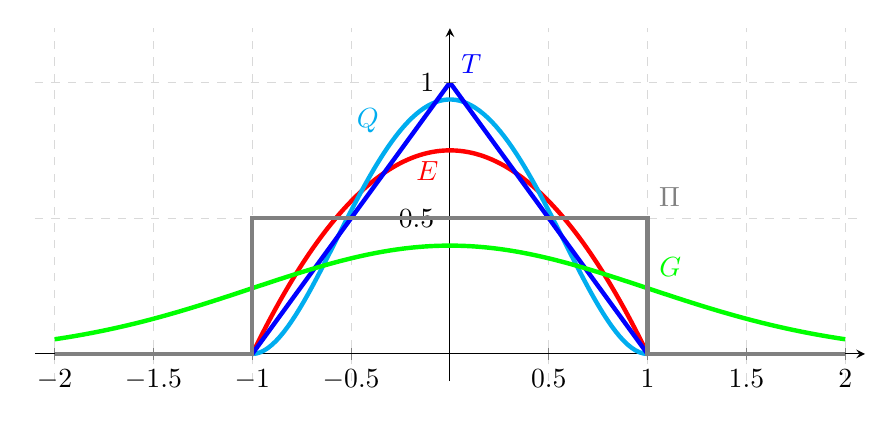
\begin{tikzpicture}
\begin{axis}[
  axis lines=center,
  width=\linewidth,
  height=0.5\linewidth,
  grid=major,
  grid style={dashed, gray!30},
  xmin=-2.1,
  xmax=2.1,
  ymin=-0.1,
  ymax=1.2
]

\addplot[domain=-1:1,samples=100,ultra thick,red] {3 / 4 * (1 - x^2)}
  node [pos=0.5, below left] {$E$};
\addplot[domain=-2:-1,samples=2,ultra thick,red] {0};
\addplot[domain=1:2,samples=2,ultra thick,red] {0};

\addplot[domain=-1:1,samples=100,ultra thick,cyan] {15 / 16 * (1 - x^2)^2}
  node [pos=0.375, above left] {$Q$};
\addplot[domain=-2:-1,samples=2,ultra thick,cyan] {0};
\addplot[domain=1:2,samples=2,ultra thick,cyan] {0};

\addplot[domain=-1:1,samples=100,ultra thick,blue] {1 - abs(x)}
  node [pos=0.5, above right] {$T$};
\addplot[domain=-2:-1,samples=2,ultra thick,blue] {0};
\addplot[domain=1:2,samples=2,ultra thick,blue] {0};

\addplot[domain=-2:2,samples=200,ultra thick,green] {1/sqrt(2 * pi) * e^(- 1 / 2 * x^2)}
  node [pos=0.75, above right] {$G$};

\addplot+[const plot, no marks, ultra thick, gray] coordinates {(-2, 0) (-1, 0) (-1, 1/2) (1, 1/2) (1, 0) (2, 0)}
  node [pos=0.7, above right] {$\Pi$};

\end{axis}
\end{tikzpicture}
\caption{Наиболее распространённые виды ядер.}\label{kde:kernels}
\end{figure}

Заметим, что в случае гауссовского ядра
формулы~\eqref{kde:features}~и~\eqref{kde:metric} совпадают.

Отметим также, что ядро Епанечникова называют также \emph{оптимальным},
поскольку оценка, полученная с его помощью даёт минимум функции риска
\[
J(K) = \int_{-\infty}^{+\infty} \E[ (\hat{p}_h(x) - p(x))^2 ] dx.
\]
Прочие ядра имеют следующие асимптотические значения функционала $J(K)/J(E)$ при
$\ell \to \infty$:
\begin{center}
\begin{tabular}{|l|l|c|}
\hline
\textbf{Ядро} $K(r)$ & \textbf{Степень гладкости} & $J(K)/J(E)$ \\
\hline
Епанечникова & $\hat{p}_h'$ разрывна & 1.000\\
Квартическое & $\hat{p}_h''$ разрывна & 0.995\\
Треугольное & $\hat{p}_h'$ разрывна & 0.989\\
Гауссовское & $\hat{p}_h\in C^\infty$ & 0.961\\
Прямоугольное & $\hat{p}_h$ разрывна & 0.943\\
\hline
\end{tabular}
\end{center}
Таким образом, поскольку ядра мало отличаются по качеству, на практике обычно
используется гауссовское ядро, в силу удобства вычислений с ним.

\subsection*{Ширина окна}
\begin{wrapfigure}{R}{0.3\textwidth}
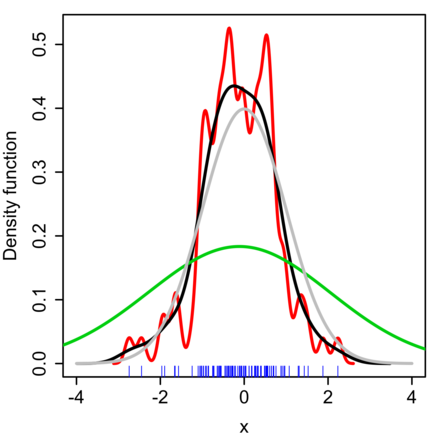
\includegraphics[width=0.3\textwidth]{chapters/bayesian/kde_bandwidth.png}
\caption{Зависимость оценки плотности от ширины окна.}\label{kde:bandwidth}
\end{wrapfigure}

На Рис.~\ref{kde:bandwidth} показаны оценки Парзена-Розенблатта с шириной окна
$h=0.05$ (красный график), $h=0.337$ (чёрный график) и $h=2$ (зелёный график)
для 100 точек из стандартного нормального распределения (серый график). При
малых $h$ заметно переобучение, при больших --- недообучение. Таким образом,
качество восстановления плотности в основном зависит от ширины окна.

\newpage
\subsection*{Задачи}

\begin{problem}
Пусть $X^\ell$ --- выборка из равномерного на отрезке $[0,1]$ распределения.
Будем использовать прямоугольное ядро и $0 < h < \frac{1}{2}$. Найдите
$\tilde{p}_h(x) = \E[\hat{p}_h(x)]$. Как влияет параметр $h$ на точность
приближения в среднем?
\end{problem}

\begin{solution}
\begin{multline*}
\tilde{p}_h(x) = \E[\hat{p}_h(x)]
  = \E\left[\frac{1}{2h\ell}\sum_{i = 1}^\ell [|x_i - x| < h]\right]\\
  = \frac{1}{2h\ell}\sum_{i = 1}^\ell P\{x_i \in [x - h, x + h]\}
  = \frac{1}{2h \cancel{\ell}} \cdot \cancel{\ell} \cdot P([0, 1] \cap [x - h, x + h]).
\end{multline*}
Итого, получаем
\begin{equation*}
\tilde{p}_h(x) =
\begin{cases}
\frac{h + x}{2h}, x \in [-h, h);\\
1, x \in [h, 1 - h];\\
\frac{1 + h - x}{2h}, x \in (1 - h, 1 + h];\\
0, x \in (-\infty, -h) \cup (h, +\infty).
\end{cases}
\end{equation*}

Высокие значения параметра $h$ <<сглаживают>> функцию, ухудшая среднюю оценку.
\end{solution}

\begin{problem}
Рассмотрим задачу бинарной классификации. Пусть объекты первого класса
распределены равномерно на отрезке $[0, 1]$, второго --- равномерно на отрезке
$[2, 3]$. Приведите значение ширины окна $h$, при котором на основе оценки
Парзена-Розенблатта с прямоугольным ядром нельзя будет построить разделяющую
поверхность между классами.
\end{problem}

\begin{solution}
Достаточно найти $h$ такой, что все точки на отрезке $[1, 2]$ не
являются точками локального минимума функции $\tilde{p}_h$. Нетрудно увидеть, что
при $h=1$ функция $\tilde{p}_h$ будет постоянной на отрезке $[0, 3]$ и иметь
в этих точках глобальный максимум.
\end{solution}

\begin{problem}
Пусть $X^\ell$ --- выборка из абсолютно непрерывного распределения с 
функцией распределения $F$. Обозначим $p_h(x) = \frac{1}{2h}P[x - h, x + h]$.
Мы знаем, что $p_h(x)~\to~p(x)~=~F'(x)$ при $h \to 0$. Докажите
\[
T_\ell = \sup_x |\hat{p}_h(x) - p_h(x)| \asto 0,\,\ell \to \infty.
\]
Сделайте вывод о сильной состоятельности оценки Парзена-Розенблатта.

\textit{
Указание: воспользуйтесь теоремой Гливенко-Кантелли из курса математической
статистики.
}
\end{problem}

\begin{solution}
Пусть $F^*_\ell(x) = \frac{1}{\ell}\sum_{i = 1}^{\ell} [x_i \leq x]$ --- эмпирическая
функция распределения. По теореме Гливенко-Кантелли имеем
\[
D_\ell = \sup_x |F^*_\ell - F(x)| \asto 0,\, \ell \to \infty.
\]

Из абсолютной непрерывности распределения и свойств функции распределения получаем
\[
p_h(x) = \frac{P[x - h, x + h]}{2h} = \frac{P(x - h, x + h]}{2h} = \frac{F(x + h) - F(x - h)}{2h}.
\]

В то же время
\[
\hat{p}_h(x) = \frac{F^*_\ell(x + h) - F^*_\ell(x - h)}{2h}.
\]

Объединяя равенства, получаем
\begin{multline*}
T_\ell
  = \sup_x |\hat{p}_h(x) - p_h(x)|
  = \sup_x \left|\frac{F^*_\ell(x + h) - F^*_\ell(x - h) - F(x + h) + F(x - h)}{2h}\right|\\
  \leq \sup_x \frac{|F^*_\ell(x + h) - F(x + h)| + |F^*_\ell(x - h) - F(x - h)|}{2h}
  \leq \frac{2 D_\ell}{2h} \asto 0.
\end{multline*}

Из $T_\ell \asto 0$ получаем также $|\hat{p}_h(x) - p_h(x)| \asto 0$ для всех $x$,
откуда заключаем, что $\hat{p}_h(x)$ --- сильно состоятельная оценка $p_h(x)$.
\end{solution}
}
